\documentclass[titlepage]{article}
\usepackage{fancyhdr}
\usepackage{hyperref}
\usepackage{graphicx}
\usepackage[font=itshape]{quoting}
\usepackage{pgfplots}
\usepackage{float}
\usepackage{amsmath}
\usepackage{tikz}
\usetikzlibrary{datavisualization}
\usepackage{listings}
\usepackage{xcolor}
\usepackage[font=itshape]{quoting}
\definecolor{codegreen}{rgb}{0,0.6,0}
\definecolor{codegray}{rgb}{0.5,0.5,0.5}
\definecolor{codepurple}{rgb}{0.58,0,0.82}
\definecolor{backcolour}{rgb}{0.95,0.95,0.92}
\definecolor{lightgray}{rgb}{0.95, 0.95, 0.95}
\definecolor{darkgray}{rgb}{0.4, 0.4, 0.4}
\definecolor{purple}{rgb}{0.65, 0.12, 0.82}
\definecolor{ocherCode}{rgb}{1, 0.5, 0} % #FF7F00 -> rgb(239, 169, 0)
\definecolor{blueCode}{rgb}{0, 0, 0.93} % #0000EE -> rgb(0, 0, 238)
\definecolor{greenCode}{rgb}{0, 0.6, 0} % #009900 -> rgb(0, 153, 0) 
% TODO: Von neumann archtecture in an appendix
\lstdefinestyle{mystyle}{
    commentstyle=\color{codegreen},
    keywordstyle=\color{magenta},
    numberstyle=\tiny\color{codegray},
    stringstyle=\color{codepurple},
    basicstyle=\ttfamily\footnotesize,
    breakatwhitespace=false,         
    breaklines=true,                 
    captionpos=b,                    
    keepspaces=true,                 
    numbers=left,                    
    numbersep=5pt,                  
    showspaces=false,                
    showstringspaces=false,
    showtabs=false,                  
    tabsize=2
}
\lstset{style=mystyle}

\newcommand{\comment}[1]{}

\pagestyle{fancy}
\fancyhf{}
\rhead{Neural Networks}
\lhead{Oliver Temple EMC Project Report}
\cfoot{\thepage}

\title{Neural Networks}

\author{Oliver Temple}
\date{March 8, 2022}
\begin{document}
\maketitle

\begin{abstract}
    Now commonplace in todays world, neural networks are becoming increasingly popular. This paper will explore the basic concepts behind neural networks, their history, how they are used in the real world and how the most simple neural networks work at a low level. The paper will conclude by exploring how to code a neural network from scratch to recognize hand written digits from 0-9.

    Neural networks are complex computational models that have many uses. Every one of the numerous different types of neural networks each has its own pros and cons which suits it for one or another of many possible tasks including computer vision, classification and prediction. The structure of neural networks can vary dramatically for different models, allowing for a wide range of applications. The fluidity of neural network structure allows them to adapt to a wide range of tasks.
    
    % Activation functions, loss functions, number of layers and neurons are just a few of the structure parameters that can be changed to create a neural network that suits the problem.
\end{abstract}
\tableofcontents
\newpage
\section{Introduction}
\subsection{What is a neural network?}
A neural network is a complex computational model that can be used to perform a wide range of tasks, such as pattern recognition, image recognition, speech recognition, and computer vision. Neural networks are constructed from a set of interconnected neurons, which are capable of processing and responding to inputs and producing outputs. A representation of a neural network is shown in Figure~\ref{fig:neural_network}.

\begin{figure}[h!]
    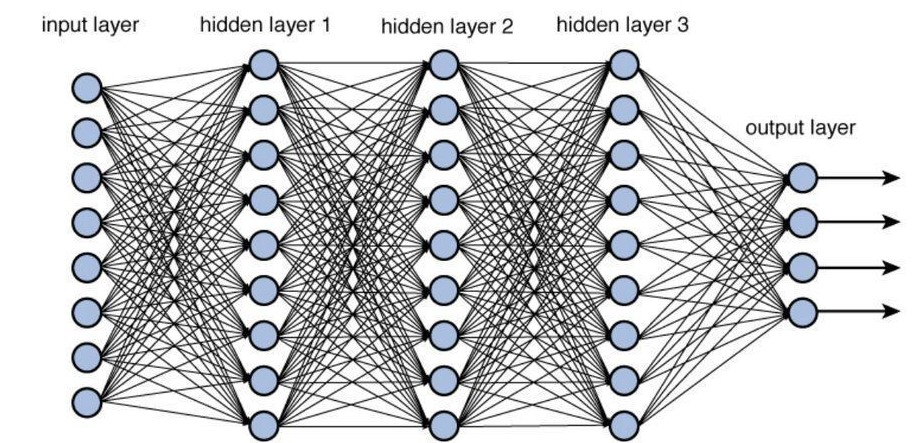
\includegraphics[width=\textwidth]{./assets/neural_network.jpeg}
    \caption{Neural Network}
    \label{fig:neural_network}
\end{figure}

\subsection{Project Goal}
The goal of this project is to explore how neural networks work at the most basic level. This will be done by researching the basic concepts behind them and using the knowledge gained to code a neural network from scratch to recognize hand written digits from 0-9 using the MNIST (Modified National Institute of Standards and Technology) dataset.

\subsection{Uses of neural networks}
In today's society, neural networks are used constantly to classify and predict a multitude of things. A common application is in social media, where complex models are used to predict which content the user will like, with the goal of increasing the user's time spent on the application.
\\\\\
More recently, neural networks have been used to assist scientists in creating hypotheses\cite{AI-hypotheses}. A team of scientists that are researching new battery technologies used a neural network to find material combinations that are more likely to work. This has saved the team a great deal of time and money, as the number of material combinations to test has been reduced.

\subsection{Different types of neural networks}
There are many different types of neural networks, and each type has its own properties that make them more specialized and useful. The most common types of neural networks are:
\begin{itemize}
    \item Perceptron
    \item Feed Forward Neural Network
    \item Multi-Layer Perceptron
    \item Convolutional Neural Network
    \item Recurrent Neural Network
    \item Long Short-Term Memory
\end{itemize} 
All the different network types described below would of course be implemented in software, as part of a computer program. When modeling a neural network using software, it can have a number of different inputs $x_1, x_2, x_3 ... x_n$, which are assembled into a vector $\textbf{x}=\begin{bmatrix}x_1\\x_2\\x_3\\\vdots\\x_n\end{bmatrix}$. Likewise, the weights are also assembled into a vector (or a matrix in the case of more complicated models) $\textbf{W}=\begin{bmatrix}w_1\\w_2\\w_3\\\vdots\\w_n\end{bmatrix}$ or $\textbf{W}=\begin{bmatrix}w_{11}&w_{12}&w_{13}&\dots&w_{1n}\\w_{21}&w_{22}&w_{23}&\dots&w_{2n}\\w_{31}&w_{32}&w_{33}&\dots&w_{3n}\\\vdots&\vdots&\vdots&\ddots&\vdots\\w_{n1}&w_{n2}&w_{n3}&\dots&w_{nn}\end{bmatrix}$.
\subsubsection{Perceptron}
A perceptron model, often referred to as a neuron, shown in Figure~\ref{fig:perceptron}, is one of the simplest and oldest neural networks. It is the smallest unit of a neural network. It accepts inputs ranging between 0 and 1, and uses the weight that each connection has to calculate the output of the neuron by taking the vector dot product (Equation~\ref{eq:vector-dot-product}) of the weights and the inputs:
\begin{equation}
    \textbf{y} = \sigma(\textbf{W}\cdot\textbf{x} + b)
    \label{eq:perceptron}
\end{equation}
Where $\textbf{y}$ is the output, $\textbf{W}$ is a vector of the weights, $\textbf{x}$ is a vector of the inputs, $b$ is the bias and $\sigma$ is the activation function.

\begin{figure}[h!]
    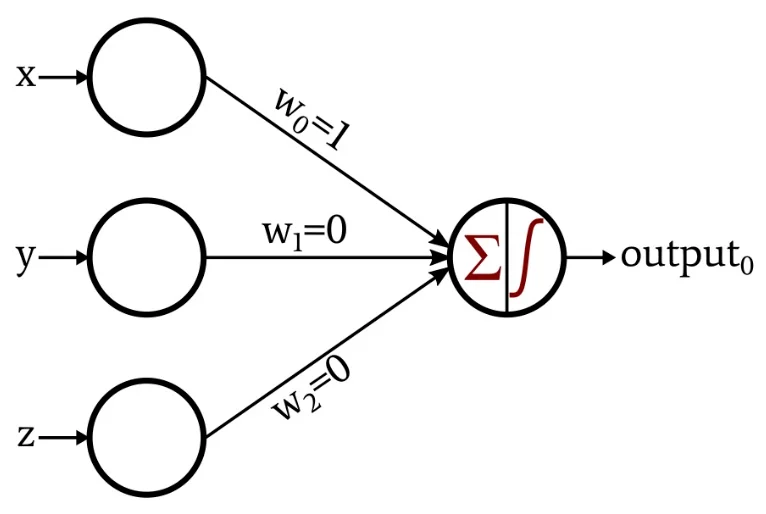
\includegraphics[width=\textwidth]{./assets/perceptron.png}
    \caption{Perceptron}
    \label{fig:perceptron}
\end{figure}

\subsubsection{Feed Forward Neural Network}
A feed forward neural network is a neural network that is constructed from a set of interconnected layers. Each neuron in a layer is connected to all of the neurons in the previous layer, and the output of each layer is used as the input to the next layer. The data travels in only one direction, making them useful only for linear classification. Each connection has a weight, and each neuron has a bias, which are used to calculate the output of the network.
\begin{equation}
    \textbf{y}_n=\sigma{(\textbf{W}_n\cdot\textbf{y}_{n-1} + \textbf{b}_n)}
    \label{eq:feed-forward}
\end{equation}
Where $\textbf{y}_n$ is the output vector of the nth layer, $\textbf{W}_n$ is the weight matrix of the nth layer, $\textbf{y}_{n-1}$ is the output vector of the previous layer, $\textbf{b}_n$ is the bias vector of the nth layer, and $\sigma$ is the activation function.

\subsubsection{Multi-Layer Perceptron}
A multi-layer perceptron is much like a feed forward neural network, in the sense that it is made up of interconnected layers of neurons, however, the data can travel both forwards and backwards through the network allowing for the network to be trained. The process in which the data travels backwards through the network is called back propagation and involves the altering of the weights and biases of the network. The output of the network is calculated the same as a feed forward network (See equation~\ref{eq:feed-forward} and Figure~\ref{fig:neural_network}).

\subsubsection{Convolutional Neural Network}
A convolutional neural network\cite{convolutionalnn} (shown in Figure~\ref{fig:convolutional_neural_network}) is often used for image recognition and contains a three dimensional arrangement of neurons. Each neuron on the first layer only processes information from a small part of the field of view. We will not be using a convolutional neural network in this project, as a multi-layer perceptron will suffice.

\begin{figure}[h!]
    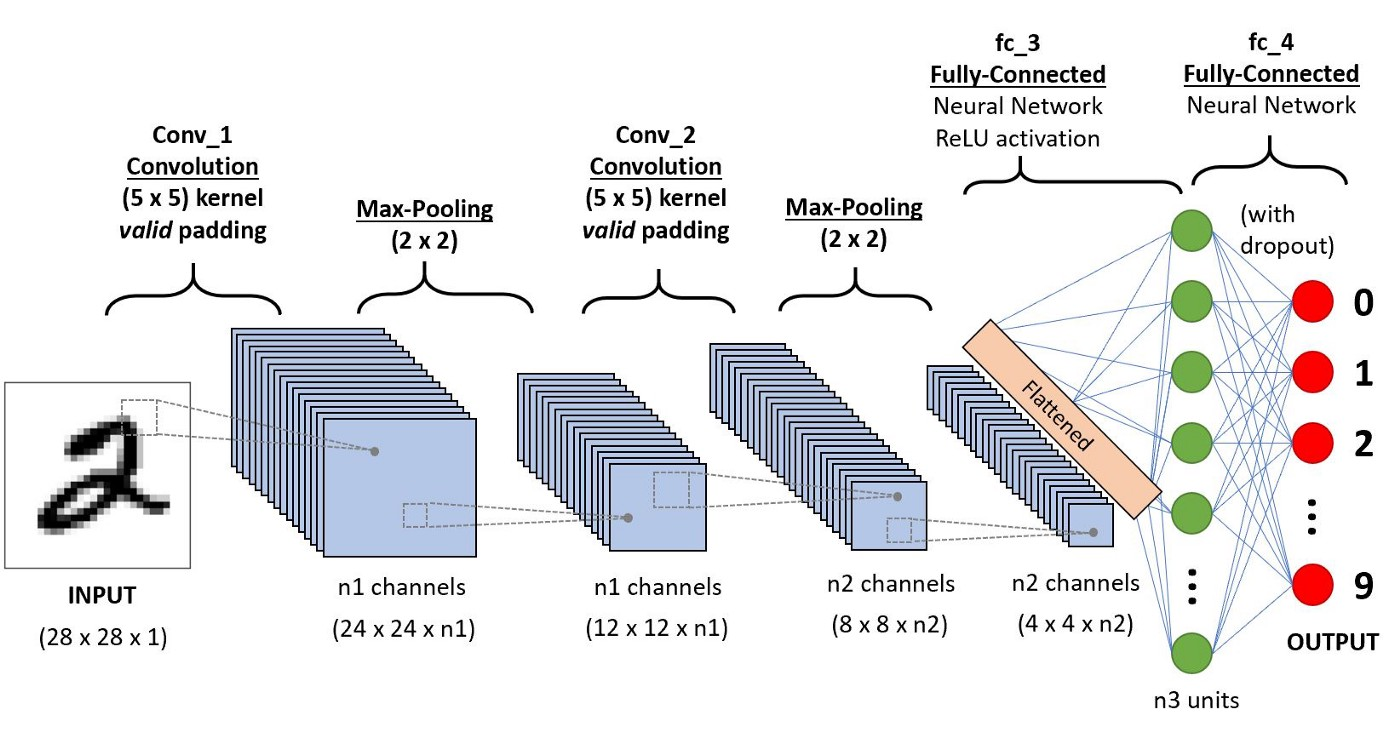
\includegraphics[width=\textwidth]{./assets/convolutional2.jpeg}
    \caption{Convolutional Neural Network}
    \label{fig:convolutional_neural_network}
\end{figure}

\subsubsection{Recurrent Neural Network}
In a recurrent neural network, the output of a layer is saved and fed back into the input to help with prediction. This is used for time series prediction, where the network can learn to predict the future. For example, given historical data, the network can attempt to predict the future.

\subsubsection{Long Short-Term Memory}
A Long Short-Term Memory (LSTM) neural network is a recurrent neural network that uses a long term memory to predict the future. LSTM neurons include a memory cell that can maintain information for long periods of time. A set of gates are used to control when information enters the memory, when it is output, and when it is forgotten.

\subsection{Motivation}
Artificial Intelligence is a field of study that is developing rapidly. The vast uses for AI make it extremely diverse and a very useful topic to understand. As neural networks are one of the most common forms of AI, I believe that this project will give me an insight into how they work, as well as a better understanding of their applications. 

\newpage
\section{The History of Neural Networks}\cite{History of Neural Networks}
Research into neural networks first began in the 1940s, when scientists were trying to explain how neurons in the brain might work. In 1943, neurophysiologist Warren McCulloch and mathematician Walter Pitts wrote a paper on how neurons might work, modeling a simple neural network using electrical circuits.
\\\\
In 1949, Donald Hebb wrote "The Organization of Behavior", which discussed how neural pathways are strengthened, a concept that is essential to how humans learn, and is often summarized as "Cells that fire together, wire together".
\\\\
In the 1950s, with improved computation power, Nathanial Rochester from the IBM research laboratories attempted to simulate a hypothetical neural network, however he failed to do so.
\\\\
In 1959, Bernard Widrow and Marcian Hoff from Stanford developed the first neural network that was applied to a real world problem. They developed two models called "ADALINE" and "MADALINE" - Multiple ADAptive LINear Elements. ADALINE was developed to recognize binary patterns, so that if it was reading streaming bits from a phone line, it could predict the next bit. MADALINE was the first neural network to be used to solve a real world problem. It used an adaptive filter that eliminated echos on phone lines and is still in commercial use.
\\\\
In 1962, Widrow and Hoff developed a learning procedure that was based on the idea that one active perceptron might have a large error, but one could then adjust the weight values to distribute the error across the network. Applying this rule does not eliminate the error if the input before the weight is 0, however the error will eventually correct itself. If the error is distributed across all of the weights, the error will be eliminated. The procedure that was developed can be written as:
\begin{equation} \label{eq:Widrow-Hoff}
    \texttt{Weight Change} = \texttt{Pre-Weight line value}\times \frac{\texttt{Error}}{\texttt{Number of Inputs}}
\end{equation}
Where error is calculated by comparing the output and the desired output (the label from the dataset).
\\\\
Despite the success that neural networks achieve later, traditional von Neumann architecture took over the computing scene, and neural network research was left behind, even though von Neumann himself suggested the imitation of neural functions by using telegraph relays or vacuum tubes.
\\\\
At the same time, a paper was published that suggested that neural networks could not be extended to more that one layer. Futhermore, many people in the field were using a learning function that was fundamentally flawed. As a result, research and funding decreased dramatically.
\\\\
Adding to this, the early success of some neural networks led to an exaggeration of the potential of neural networks, leading to promises that could not be fulfilled. Furthermore, philosophical questions led to fear, with writers pondering the effect that the so-called "thinking machines" would have on humanity, ideas which are still around today.
\\\\
In 1982, John Hopfield of Caltech published a paper theorising that connections between neurons could be two way, instead of the one way that they had been until this point. This paper renewed interest in the field. This was coupled with Reilly and Cooper using a "Hybrid Network" in the same year, with multiple layers using different problem solving strategies.
\\\\
Also in 1982, at a US-Japan conference, Japan announced a new effort on neural networks, and US papers generated worry that the US could be left behind. This led to more funding and more research in the field.
\\\\
In 1986, with more research into multi-layer neural networks, the problem was how to extend the Widrow-Hoff rule (equation~\ref{eq:Widrow-Hoff}) to multiple layers. Three independent groups of researchers came up with similar ideas, which are now called back propagation networks, which used many layers and are slow learners, needing possibly thousands of iterations lo learn.
\\\\
In modern technology, neural networks are used in many applications. The fundamental idea behind the nature of neural networks is that if it works in nature, it must be able to work on computers.
\newpage
\section{Bias in Artificial Intelligence}
Despite the many benefits of neural networks, there are still many problems that are not solved. The most common problem is that bias in the training data can cause bias in the predictions of the network. However, societal bias is also an issue, where our assumptions and norms as a society cause us to have blind spots in our thinking. These biases usually reflect widespread societal biases about race, gender, biological sex, age and culture. \cite{Bias in Artificial Intelligence}
\subsection{What causes bias in AI?}
\subsubsection{Data Bias}
As stated above, bias in AI can be caused by a bias in the training data. For example, an AI model that is being trained to detect faces, could be trained with more photos of a specific gender or race, making it better at detecting that group of people.

\subsubsection{Societal Bias}
Many people think that computers are impartial, and while this is true for your microwave oven or your vacuum cleaner, a computer that can "think" may not be impartial. Take humans for example; upbringing, experiences and culture are just some of the things that shape people, and they internalize certain assumptions about the world around them. AI is much the same. Algorithms built by humans can show the bias of the people who built them. AIs tend to "think" the way they have been taught. The algorithms and data that outputs the biased results often appear unbiased, but their outputs show that the bias is present. 

\subsection{Examples of Bias in AI}
\subsubsection{PortraitAI Art Generator}
The portrait AI art generator, \url{https://ai-art.tokyo/en/}, takes an image, and renders an image of the user in the manner of Baroque and Renaissance art. The results are great for white people, however, due to most of the paintings from this era being of white Europeans, the training data would have been biased towards white people.
\\\\
The company who owns the service has said:
\begin{quoting}
    Currently, the AI portrait generator has been trained mostly on portraits of people of European ethnicity. We're planning to expand our dataset and fix this in the future. At the time of conceptualizing this AI, authors were not certain it would turn out to work at all. This generator is close to the state-of-the-art in AI at the moment. Sorry for the bias in the meanwhile. Have fun!
\end{quoting}

\subsubsection{Twitter Photo Cropping}
Despite the size of a company like Twitter, AI bias is still an issue. Twitter recently apologized after uses claimed that its image-cropping algorithm was racist. The goal of the algorithm is to crop the image, centering on a human face. However, it only works if you're white (and more so if you're male). If your image contained a white person and a black person, the white person would be centered in the preview. Even animal and cartoon faces received preferential treatment over black faces. In response, a Twitter spokesperson said:
\begin{quoting}
    Our team did test for bias before shipping the model and did not find evidence of racial or gender bias in our testing. But it's clear from these examples that we've got more analysis to do. We'll continue to share what we learn, what actions we take, and will open source our analysis so others can review and replicate.
\end{quoting}
\newpage
\section{How Neural Networks Work}
At its core, a neural network is a collection of neurons, formed into layers, that are all interconnected. Each neuron has its own bias, and each connection has a weight. These parameters are what determine the output of the network. Although the diagrams below, and the concepts they portray imply a discrete physical implementation of each neuron interconnected by wires or some sort of physical signal path, in practice the neurons are implemented in software. The interconnections are implemented in practice by the passing of variables carrying the relevant information from one part of the program to another.

\begin{figure}[h!]
    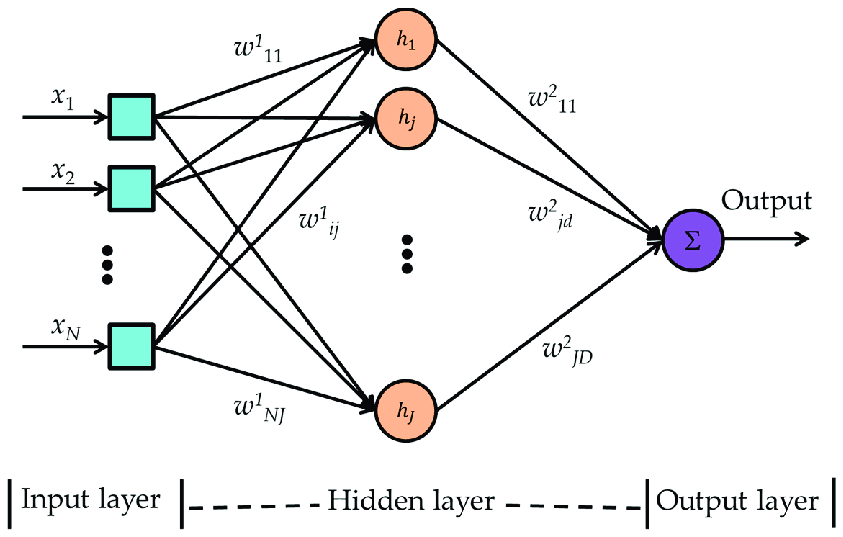
\includegraphics[width=\textwidth]{assets/multilayer perceptron.png}
    \caption{Multilayer Perceptron}
    \label{fig:multilayer-perceptron}
\end{figure}
\subsection{Structure}
The output implementation selects the highest output from the neurons in the final layer and discards the rest, but in successive tasks it may well be (indeed is likely) that different neurons will provide this highest output and it might have different values. The structure of the network is the first thing that must be defined. The input layer must consist of the same number of neurons as there are data points (e.g. one neuron per pixel in an image), and the output layer must consist of the same number of neurons as there are classification labels (the total number of outputs). There can be any number of hidden layers, which can have any number of neurons. The size and number of hidden layers should be varied to determine what sizes give the best results for the problem.
% For my project I will be using a multilayer perceptron (Figure~\ref{fig:multilayer-perceptron}) as it allows for back propagation to be used, while not becoming to complex, like a convolutional neural network.

\subsection{Forward Propagation}
The purpose of forward propagation is to get an output (or prediction) from our neural network. To calculate it we use the vector dot product (Appendix~\ref{eq:vector-dot-product}) of the inputs and the weights, and add the bias. The output of the $n^{th}$ layer can be calculated using the formula in the equation~\ref{eq:forward-propagation}.
\begin{equation}
    \textbf{y}_n = \sigma{(\textbf{W}_n\cdot\textbf{y}_{(n-1)} + \textbf{b}_n)}
    \label{eq:forward-propagation}
\end{equation}
where $\textbf{W}_n$ is a matrix of the weights for the $n^{th}$ layer, $\textbf{y}_{(n-1)}$ is the output vector of the previous layer (the input of the network for the fist layer) and $\textbf{b}_n$ is a vector of the biases for the $n^{th}$ layer.


\subsection{Activation Functions}
The activation function is applied to the output of each neuron before it is inputted into the next layer. The purpose of an activation function is to prevent the input from being too high or too low, and to add some non-linearity to the network. There are many different activation functions to choose from, some of the more common ones are:
\begin{itemize}
    \item Sigmoid
    \item Tanh
    \item ReLU
    \item Leaky ReLU
\end{itemize}
\subsubsection{Sigmoid}
The sigmoid function(Figure~\ref{fig:sigmoid_function}) takes any input, $x$ and translates it to a value between 0 and 1. The equation is:
\begin{equation}
    \sigma(x) = \frac{1}{1 + e^{-x}}
    \label{eq:sigmoid}
\end{equation}
\begin{figure}[h!]
    \begin{center}
        \begin{tikzpicture}
            \begin{axis}[axis x line=bottom, axis y line=middle, xmin=-6, xmax=6, xlabel={$x$}, ylabel={$\sigma(x)$}]
            \addplot[color=red]{1/(1+exp(-x))};
            \end{axis}
        \end{tikzpicture}
    \end{center}
    \caption{Sigmoid Function}    
    \label{fig:sigmoid_function}
\end{figure}


\subsubsection{Tanh}
Similar to the sigmoid function, the tanh function(Figure~\ref{fig:tanh}) takes any input, $x$ and translates it to a value between -1 and 1. The equation is:
\begin{equation}
    \tanh(x) = \frac{e^{x} - e^{-x}}{e^{x} + e^{-x}}
    \label{eq:tanh}
\end{equation}
\begin{figure}[h!]
    \begin{center}
        \begin{tikzpicture}
            \begin{axis}[axis x line=bottom, axis y line=middle, xmin=-6, xmax=6, xlabel={$x$}, ylabel={$\tanh(x)$}]
            \addplot[color=red]{tanh(x)};
            \end{axis}
        \end{tikzpicture}
    \end{center}
    \caption{Tanh Function}    
    \label{fig:tanh}
\end{figure}


\subsubsection{ReLU}
Unlike the sigmoid function and the $\tanh$ function, the ReLU function(Figure~\ref{fig:relu}) takes any input, $x$ and if it is negative, it returns 0, otherwise it returns the input. The equation is:
\begin{equation}
    \texttt{ReLU}(x) = \max(0, x)
    \label{eq:relu}
\end{equation}

\begin{figure}[h!]
    \begin{center}
        \begin{tikzpicture}
            \begin{axis}[axis x line=bottom, axis y line=middle, xmin=-6, xmax=6, xlabel={$x$}, ylabel={$\texttt{ReLU}(x)$}]
            \addplot[color=red]{max(0, x)};
            \end{axis}
        \end{tikzpicture}
    \end{center}
    \caption{ReLU Function}  
    \label{fig:relu}
\end{figure}

\subsubsection{Leaky ReLU}
The Leaky ReLU function(Figure~\ref{fig:leaky-relu}) takes any input, $x$ and if it is negative, it returns a scaled down input, otherwise it returns the input. The equation is:
\begin{equation}
    \texttt{Leaky ReLU}(x) = \max(0.1x, x)
    \label{eq:leaky-relu}
\end{equation}
\begin{figure}[h!]
    \begin{center}
        \begin{tikzpicture}
            \begin{axis}[axis x line=middle, axis y line=middle, xmin=-6, xmax=6, xlabel={$x$}, ylabel={$\texttt{Leaky ReLU}(x)$}]
            \addplot[color=red]{max(0.1*x, x)};
            \end{axis}
        \end{tikzpicture}
    \end{center}
    \caption{Leaky ReLU Function}    
    \label{fig:leaky-relu}
\end{figure}

\subsection{Loss Function}
The loss function is used to calculate how good a model is. In order to calculate the loss we need the output of our network, and the expected output\cite{Loss Functions}. Similar to activation functions, there are many different loss functions to choose from. Two of the more common ones are:
\begin{itemize}
    \item Mean Squared Error (MSE)
    \item Cross Entropy Loss (or Log Loss)
\end{itemize}

\subsubsection{Mean Squared Error}
The MSE loss function is calculate as the average of the squared difference between the network's output and the desired output. The equation is:
\begin{equation}
    \texttt{MSE} = \frac{1}{n} \sum_{i=1}^{n} (\hat{y}_i - y_i)^2
    \label{eq:MSE}
\end{equation}
where $n$ is the number of samples we are testing against, $y$ is the desired output of the network, and $\hat{y}$ is the actual output of the network.

\subsubsection{Cross Entropy Loss}
Cross entropy loss, often called log loss, is a loss function that is used for more complex models. Each predicted output is compared to the desired output and a score is calculated that penalizes the output based on the difference between the two. The penalty is logarithmic, meaning smaller score for smaller differences, and larger score for larger differences. The equation is:
\begin{equation}
    \texttt{CEL} = -\frac{1}{n}\sum_{i=1}^{n}(y_i\times\log(\hat{y}_i))
    \label{eq:CEL}
\end{equation}
where $n$ is the number of samples we are testing against, $y$ is the desired output of the network, and $\hat{y}$ is the actual output of the network.

\subsection{Backpropagation}
Backpropagation is the process in which the data moves backwards through the network, adjusting the weights and biases to minimize the loss function. To do so, the derivative of the loss function must first be calculated, as this will allow us to know whether to increase or decrease the weights and biases, and by how much.
\begin{figure}[h!]
    \begin{center}
        \begin{tikzpicture}
            \begin{axis}[axis x line=middle, axis y line=middle, xlabel={Weight}, ylabel={Loss}]
            \addplot[color=red]{x*x};
            \end{axis}
        \end{tikzpicture}
    \end{center}
    \caption{Loss against Weight}
    \label{fig:loss-vs-weights}
\end{figure}
\\\\
For example, if a graph of loss against weights is plotted, as seen in Figure~\ref{fig:loss-vs-weights}, the minimum of the function is calculated using the derivative. However, as the loss function is usually in many more dimensions, the minimum cannot be calculated exactly, and small steps towards the minimum are required. 
\\\\
When we have the derivative of the loss function, we know whether to increase or decrease the weights and biases due to the sign of the gradient. The weights and biases can be changed proportionally to the gradient to prevent missing the minimum of the function.
\\\\
This process is repeated many times over the course of training, with the goal of setting the weights and biases to the values that give the lowest loss of the network.
\subsection{Training}
In order for a network to be used to classify data, it must first be trained. Before we can train the network, we must first initialize the weights and biases with small random values. Next, we must split our dataset into training data and testing data, so that once training has been completed we can test the model on unseen data to get an idea of how it would perform in the real world. Training a network is done through the following process:
\begin{enumerate}
    \item Propagate all the values in the input layer through the network (Forward Propagation).
    \item Update the weights and biases of the network using the loss function (Back Propagation).
    \item Repeat until the accuracy of the network is satisfactory.
\end{enumerate}
\newpage
\section{Coding a Neural Network}
\subsection{Data}
When training a neural network, one of the most important assets is the data that will be used to train and test the neural network. Any imperfections in the data, such as incorrect labels or biases will be reflected in the output of the network, so it important to use a dataset you know to be accurate and unbiased. For my project, I will be using the MNIST dataset, which is a set of labelled hand written digits from 0-9. The images are represented as a list of 784 monochromatic pixels (28x28 pixel images) with values between 0 and 255 to represent the the brightness of the pixel. Before the images can be used, they must be normalized to be between 0 and 1. To do this, we divide every number by 255, to get a floating point representation of the pixel data.
\subsection{Splitting the Data}
When creating a neural network it is important to split our data set into a "train" set and a "test" set. This is so that we can test our neural network on data that it hasn't seen before, which will give us an idea of the accuracy of the model. For our model we will be using 50000 training samples and 10000 testing samples.
\subsection{Defining the Model}
Before training the model, we have to define the structure. A neural network is made up of layers of interconnected neurons, and when defining the structure of our network, we must define how many layers we want, how many neurons we want in each layer.
\subsubsection{Layers}
As the input images are 28x28, our input layer will consist of 784 neurons, allowing for each neuron to represent a single pixel. The output layer will consist of 10 neurons, one for each possible digit. We will also be using a hidden layer of 350 neurons. The size of the hidden layer can be changed, but 350 was chosen as it is between 748 and 10. If the task was more complex, more hidden layers with larger sizes could be used, however, that would not be necessary for this project, and would slow down the training process.
\subsubsection{Loss Function}
We also need to define our loss function. In this model, we will be using the Mean Squared Error (MSE Equation~\ref{eq:MSE}) loss function, as it provides a good balance between accuracy and speed.
\subsubsection{Activation Function}
Finally, we need to define our activation function, and its derivative. In this model, we will be using the sigmoid function (Equation~\ref{eq:sigmoid}), as it also provides a good balance between accuracy and speed. We also need the derivative of our activation function for back propagation. The derivative of the sigmoid function is defined in Equation~\ref{eq:sigmoid-derivative}.
\begin{equation}
    \sigma'(x) = x(1-x)
    \label{eq:sigmoid-derivative}
\end{equation}


\subsection{Training the Model}
To train the model, the data is split up into equal size batches. This saves us from running through the entire dataset multiple times. Each batch is then passed through the network, and the loss is calculated - This is called an Epoch. After each Epoch, the loss is used to backpropagate through the network. However, when training the neural network, there are several things we need to take into account. A graph of the loss over each epoch can be seen in \ref{fig:loss}
\begin{figure}[h!]
    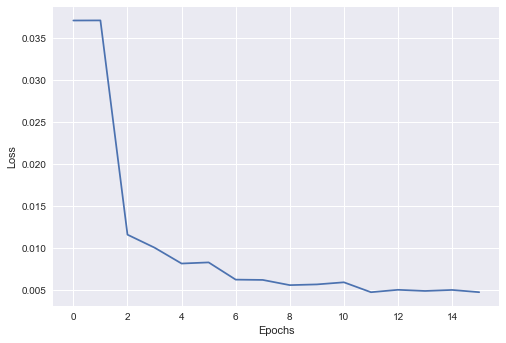
\includegraphics[width=\linewidth]{assets/loss.png}
    \caption{Loss of neural network over epochs}
    \label{fig:loss}
\end{figure}
\subsubsection{Over Fitting}
Over-fitting is when the model has been over fitted to the training data, meaning that it is very good at classifying the training data, but when it is given new data, it does not classify it well.

\subsubsection{The Curse of Dimensionality}
The optimization of neural networks has led them to make use of many dimensions for the error surface. In figure~\ref{fig:loss-vs-weights}, only one dimension is used, for simplicity, however, in real neural networks, the error surface is in many dimensions, in some cases up to millions of dimensions. This causes a problem, as the addition of each new dimension dramatically increases the distance between the points in space.\cite{curse-of-dimensionality}
\begin{quotation}
    This phenomenon is known as the curse of dimensionality. Of particular concern is that the number of possible distinct configurations of a set of variables increases exponentially as the number of variables increases
\end{quotation}

\subsubsection{Local Minima}
When minimizing the loss function, the derivative is found to calculate whether to increase the weights and bias. This does allow us to improve our model, however, it may not lead us to the optimal solution, as a local minimum may exist.
% [0.6478276249887084, 0.28551481908826687, 0.21974857429117917, 0.1758817580463027, 0.1465148527377736, 0.12774579912257283, 0.11215119620165559, 0.09928242960023378, 0.09033128010061409, 0.08122211917917103, 0.07357034309586483, 0.06754901132453034, 0.06237644694749512, 0.05664522448596336, 0.052354815337848644]

\subsection{Testing the Model}
Once our model has been trained, it is important to test it on unseen data so that we can see how well it would perform in the real world. To do this, we will run the test dataset through the neural network and check the prediction against the label for each data point in the test set. Keeping track of how many items were correctly classified allows us to calculate the accuracy of the model. The accuracy of our model was 95.32\%, calculated on a test data set of 10000 items. If we take a sample of 9 randomly selected items from the test set, we can plot the images and see where the neural network is making mistakes. The images shown in figure \ref{fig:sample-predictions} were fed into the neural network, and the predictions (output from the network) were 8, 5, 8, 9, 1, 9, 7, 2, 8 and the labels for the inputs were 5, 5, 8, 9, 1, 9, 7, 2, 8. As you can see, in this sample, the network was correct 88\% of the time, only making one error. The accuracy is lower in this sample, as only 9 items were selected.
\begin{figure}[h!]
    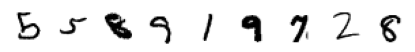
\includegraphics[width=\linewidth]{assets/sample_predictions.png}
    \caption{Sample inputs of neural network}
    \label{fig:sample-predictions}
\end{figure}
 
\subsection{Discussion of Results}
As shown in the testing, the model is not perfect. To improve the model, more layers could be added, the loss function could be altered or the activations function could be changed. If the model were to be used in a real world application, it would be important to make sure that the model was very accurate, and implementing the improvements mentioned above would be much easier if a library like tensorflow\cite{tensorflow} or pytorch\cite{pytorch} was used. They have pre-defined models that can be highly customizable, and make the process of training the model simpler as knowledge of how neural networks work from a low level is not required. 
\newpage
\section{Conclusion}
To conclude, neural networks are complex models used for many different tasks. Each of the many types of neural network has its own respective merits and downfalls. Different types of neural network will be best suited to specific tasks. Although it is possible to code them from scratch, it is much easier and quicker to use a library, as they are very well optimized, and already have complex loss and activation functions implemented as well as other types of networks.
\\\\
By completing this project, I have gained knowledge of how neural networks work from a high level (complex ideas abstracted away for simplicity), as well as how the most basic of neural networks work from a low level (including all of the details). I have also gained an understanding of what neural networks are used for as well as the history of how they came about. I have also learned about the issues that we need to be wary of when training a neural network.
\newpage
\section{Appendix}
\subsection{Vector Dot Product}
\begin{align} 
    \begin{bmatrix}
        x_1\\
        x_2\\
        x_3\\
        \vdots\\
        x_n
    \end{bmatrix}
    \cdot
    \begin{bmatrix}
        y_1\\
        y_2\\
        y_3\\
        \vdots\\
        y_n
    \end{bmatrix}
    &= \sum_{i=1}^{n} x_iy_i 
    \label{eq:vector-dot-product}
    \\
    \begin{bmatrix}
        x_{11}&x_{12}&x_{13}&\dots&x_{1n}\\
        x_{21}&x_{22}&x_{23}&\dots&x_{2n}\\
        \vdots&\vdots&\vdots&\ddots&\vdots\\
        x_{n1}&x_{n2}&x_{n3}&\dots&x_{nn}
    \end{bmatrix}
    \cdot
    \begin{bmatrix}
        y_1\\
        y_2\\
        \vdots\\
        y_n
    \end{bmatrix}
    &=
    \begin{bmatrix}
        x_{11}y_1+x_{12}y_2+\dots+x_{1n}y_n\\
        x_{21}y_1+x_{22}y_2+\dots+x_{2n}y_n\\
        \vdots\\
        x_{n1}y_1+x_{n2}y_2+\dots+x_{nn}y_n
    \end{bmatrix}
    \label{eq:vector-dot-product-2}
\end{align}
\url{https://en.wikipedia.org/wiki/Dot_product#Algebraic_definition}
\subsection{MNIST Dataset}
An example of a training sample from the dataset is shown below:
\\\\
label: 7
\\\\
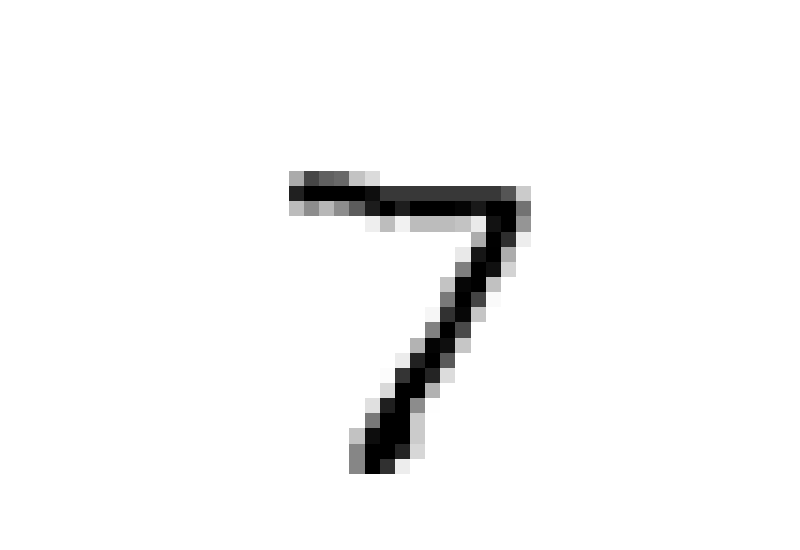
\includegraphics[width=\linewidth]{assets/mnist_example.png}
\\\\
Output of network:
[[1.31662437e-05]
 [3.42552722e-06]
 [2.50440275e-03]
 [2.50623411e-03]
 [7.89115799e-09]
 [3.33512945e-04]
 [2.93168886e-06]
 [9.99565501e-01]
 [6.19048673e-04]
 [2.45914335e-05]]
\\\\
\resizebox{\textwidth}{!}{
\begin{tabular}{c||c c c c c c c c c c}
    output & 1.3e-05 & 3.4e-06 & 0.0025 & 0.0025 & 7.9e-09 & 0.00033 & 2.9e-06 & \textbf{0.99} & 0.00062 & 2.5e-05 \\
    prediction & 0 & 1 & 2 & 3 & 4 & 5 & 6 & \textbf{7} & 8 & 9 \\
\end{tabular}}
\\\\
Prediction: 7
\\\\
pixel patterns (input to network): 
[[0.        ],[0.        ],[0.        ],[0.        ],[0.        ],[0.        ],[0.        ],[0.        ],[0.        ],[0.        ],[0.        ],[0.        ],[0.        ],[0.        ],[0.        ],[0.        ],[0.        ],[0.        ],[0.        ],[0.        ],[0.        ],[0.        ],[0.        ],[0.        ],[0.        ],[0.        ],[0.        ],[0.        ],[0.        ],[0.        ],[0.        ],[0.        ],[0.        ],[0.        ],[0.        ],[0.        ],[0.        ],[0.        ],[0.        ],[0.        ],[0.        ],[0.        ],[0.        ],[0.        ],[0.        ],[0.        ],[0.        ],[0.        ],[0.        ],[0.        ],[0.        ],[0.        ],[0.        ],[0.        ],[0.        ],[0.        ],[0.        ],[0.        ],[0.        ],[0.        ],[0.        ],[0.        ],[0.        ],[0.        ],[0.        ],[0.        ],[0.        ],[0.        ],[0.        ],[0.        ],[0.        ],[0.        ],[0.        ],[0.        ],[0.        ],[0.        ],[0.        ],[0.        ],[0.        ],[0.        ],[0.        ],[0.        ],[0.        ],[0.        ],[0.        ],[0.        ],[0.        ],[0.        ],[0.        ],[0.        ],[0.        ],[0.        ],[0.        ],[0.        ],[0.        ],[0.        ],[0.        ],[0.        ],[0.        ],[0.        ],[0.        ],[0.        ],[0.        ],[0.        ],[0.        ],[0.        ],[0.        ],[0.        ],[0.        ],[0.        ],[0.        ],[0.        ],[0.        ],[0.        ],[0.        ],[0.        ],[0.        ],[0.        ],[0.        ],[0.        ],[0.        ],[0.        ],[0.        ],[0.        ],[0.        ],[0.        ],[0.        ],[0.        ],[0.        ],[0.        ],[0.        ],[0.        ],[0.        ],[0.        ],[0.        ],[0.        ],[0.        ],[0.        ],[0.        ],[0.        ],[0.        ],[0.        ],[0.        ],[0.        ],[0.        ],[0.        ],[0.        ],[0.        ],[0.        ],[0.        ],[0.        ],[0.        ],[0.        ],[0.        ],[0.        ],[0.        ],[0.        ],[0.        ],[0.        ],[0.        ],[0.        ],[0.        ],[0.        ],[0.        ],[0.        ],[0.        ],[0.        ],[0.        ],[0.        ],[0.        ],[0.        ],[0.        ],[0.        ],[0.        ],[0.        ],[0.        ],[0.        ],[0.        ],[0.        ],[0.        ],[0.        ],[0.        ],[0.        ],[0.        ],[0.        ],[0.        ],[0.        ],[0.        ],[0.        ],[0.        ],[0.        ],[0.        ],[0.        ],[0.        ],[0.        ],[0.        ],[0.        ],[0.        ],[0.        ],[0.        ],[0.        ],[0.        ],[0.328125  ],[0.72265625],[0.62109375],[0.58984375],[0.234375  ],[0.140625  ],[0.        ],[0.        ],[0.        ],[0.        ],[0.        ],[0.        ],[0.        ],[0.        ],[0.        ],[0.        ],[0.        ],[0.        ],[0.        ],[0.        ],[0.        ],[0.        ],[0.        ],[0.        ],[0.        ],[0.        ],[0.        ],[0.        ],[0.8671875 ],[0.9921875 ],[0.9921875 ],[0.9921875 ],[0.9921875 ],[0.94140625],[0.7734375 ],[0.7734375 ],[0.7734375 ],[0.7734375 ],[0.7734375 ],[0.7734375 ],[0.7734375 ],[0.7734375 ],[0.6640625 ],[0.203125  ],[0.        ],[0.        ],[0.        ],[0.        ],[0.        ],[0.        ],[0.        ],[0.        ],[0.        ],[0.        ],[0.        ],[0.        ],[0.26171875],[0.4453125 ],[0.28125   ],[0.4453125 ],[0.63671875],[0.88671875],[0.9921875 ],[0.87890625],[0.9921875 ],[0.9921875 ],[0.9921875 ],[0.9765625 ],[0.89453125],[0.9921875 ],[0.9921875 ],[0.546875  ],[0.        ],[0.        ],[0.        ],[0.        ],[0.        ],[0.        ],[0.        ],[0.        ],[0.        ],[0.        ],[0.        ],[0.        ],[0.        ],[0.        ],[0.        ],[0.        ],[0.        ],[0.06640625],[0.2578125 ],[0.0546875 ],[0.26171875],[0.26171875],[0.26171875],[0.23046875], [0.08203125],[0.921875  ],[0.9921875 ],[0.4140625 ],[0.        ],[0.        ],[0.        ],[0.        ],[0.        ],[0.        ],[0.        ],[0.        ],[0.        ],[0.        ],[0.        ],[0.        ],[0.        ],[0.        ],[0.        ],[0.        ],[0.        ],[0.        ],[0.        ],[0.        ],[0.        ],[0.        ],[0.        ],[0.        ],[0.32421875],[0.98828125],[0.81640625],[0.0703125 ],[0.        ],[0.        ],[0.        ],[0.        ],[0.        ],[0.        ],[0.        ],[0.        ],[0.        ],[0.        ],[0.        ],[0.        ],[0.        ],[0.        ],[0.        ],[0.        ],[0.        ],[0.        ],[0.        ],[0.        ],[0.        ],[0.        ],[0.        ],[0.0859375 ],[0.91015625],[0.99609375],[0.32421875],[0.        ],[0.        ],[0.        ],[0.        ],[0.        ],[0.        ],[0.        ],[0.        ],[0.        ],[0.        ],[0.        ],[0.        ],[0.        ],[0.        ],[0.        ],[0.        ],[0.        ],[0.        ],[0.        ],[0.        ],[0.        ],[0.        ],[0.        ],[0.        ],[0.50390625],[0.9921875 ],[0.9296875 ],[0.171875  ],[0.        ],[0.        ],[0.        ],[0.        ],[0.        ],[0.        ],[0.        ],[0.        ],[0.        ],[0.        ],[0.        ],[0.        ],[0.        ],[0.        ],[0.        ],[0.        ],[0.        ],[0.        ],[0.        ],[0.        ],[0.        ],[0.        ],[0.        ],[0.23046875],[0.97265625],[0.9921875 ],[0.2421875 ],[0.        ],[0.        ],[0.        ],[0.        ],[0.        ],[0.        ],[0.        ],[0.        ],[0.        ],[0.        ],[0.        ],[0.        ],[0.        ],[0.        ],[0.        ],[0.        ],[0.        ],[0.        ],[0.        ],[0.        ],[0.        ],[0.        ],[0.        ],[0.        ],[0.51953125],[0.9921875 ],[0.73046875],[0.01953125],[0.        ],[0.        ],[0.        ],[0.        ],[0.        ],[0.        ],[0.        ],[0.        ],[0.        ],[0.        ],[0.        ],[0.        ],[0.        ],[0.        ],[0.        ],[0.        ],[0.        ],[0.        ],[0.        ],[0.        ],[0.        ],[0.        ],[0.        ],[0.03515625],[0.80078125],[0.96875   ],[0.2265625 ],[0.        ],[0.        ],[0.        ],[0.        ],[0.        ],[0.        ],[0.        ],[0.        ],[0.        ],[0.        ],[0.        ],[0.        ],[0.        ],[0.        ],[0.        ],[0.        ],[0.        ],[0.        ],[0.        ],[0.        ],[0.        ],[0.        ],[0.        ],[0.        ],[0.4921875 ],[0.9921875 ],[0.7109375 ],[0.        ],[0.        ],[0.        ],[0.        ],[0.        ],[0.        ],[0.        ],[0.        ],[0.        ],[0.        ],[0.        ],[0.        ],[0.        ],[0.        ],[0.        ],[0.        ],[0.        ],[0.        ],[0.        ],[0.        ],[0.        ],[0.        ],[0.        ],[0.        ],[0.29296875],[0.98046875],[0.9375    ],[0.22265625],[0.        ],[0.        ],[0.        ],[0.        ],[0.        ],[0.        ],[0.        ],[0.        ],[0.        ],[0.        ],[0.        ],[0.        ],[0.        ],[0.        ],[0.        ],[0.        ],[0.        ],[0.        ],[0.        ],[0.        ],[0.        ],[0.        ],[0.        ],[0.07421875],[0.86328125],[0.9921875 ],[0.6484375 ],[0.        ],[0.        ],[0.        ],[0.        ],[0.        ],[0.        ],[0.        ],[0.        ],[0.        ],[0.        ],[0.        ],[0.        ],[0.        ],[0.        ],[0.        ],[0.        ],[0.        ],[0.        ],[0.        ],[0.        ],[0.        ],[0.        ],[0.        ],[0.01171875],[0.79296875],[0.9921875 ],[0.85546875],[0.13671875],[0.        ],[0.        ],[0.        ],[0.        ],[0.        ],[0.        ],[0.        ],[0.        ],[0.        ],[0.        ],[0.        ],[0.        ],[0.        ],[0.        ],[0.        ],[0.        ],[0.        ],[0.        ],[0.        ],[0.        ],[0.        ],[0.        ],[0.        ],[0.1484375 ],[0.9921875 ],[0.9921875 ],[0.30078125],[0.        ],[0.        ],[0.        ],[0.        ],[0.        ],[0.        ],[0.        ],[0.        ],[0.        ],[0.        ],[0.        ],[0.        ],[0.        ],[0.        ],[0.        ],[0.        ],[0.        ],[0.        ],[0.        ],[0.        ],[0.        ],[0.        ],[0.        ],[0.12109375],[0.875     ],[0.9921875 ],[0.44921875],[0.00390625],[0.        ],[0.        ],[0.        ],[0.        ],[0.        ],[0.        ],[0.        ],[0.        ],[0.        ],[0.        ],[0.        ],[0.        ],[0.        ],[0.        ],[0.        ],[0.        ],[0.        ],[0.        ],[0.        ],[0.        ],[0.        ],[0.        ],[0.        ],[0.51953125],[0.9921875 ],[0.9921875 ],[0.203125  ],[0.        ],[0.        ],[0.        ],[0.        ],[0.        ],[0.        ],[0.        ],[0.        ],[0.        ],[0.        ],[0.        ],[0.        ],[0.        ],[0.        ],[0.        ],[0.        ],[0.        ],[0.        ],[0.        ],[0.        ],[0.        ],[0.        ],[0.        ],[0.23828125],[0.9453125 ],[0.9921875 ],[0.9921875 ],[0.203125  ],[0.        ],[0.        ],[0.        ],[0.        ],[0.        ],[0.        ],[0.        ],[0.        ],[0.        ],[0.        ],[0.        ],[0.        ],[0.        ],[0.        ],[0.        ],[0.        ],[0.        ],[0.        ],[0.        ],[0.        ],[0.        ],[0.        ],[0.        ],[0.47265625],[0.9921875 ],[0.9921875 ],[0.85546875],[0.15625   ],[0.        ],[0.        ],[0.        ],[0.        ],[0.        ],[0.        ],[0.        ],[0.        ],[0.        ],[0.        ],[0.        ],[0.        ],[0.        ],[0.        ],[0.        ],[0.        ],[0.        ],[0.        ],[0.        ],[0.        ],[0.        ],[0.        ],[0.        ],[0.47265625],[0.9921875 ],[0.80859375],[0.0703125 ],[0.        ],[0.        ],[0.        ],[0.        ],[0.        ],[0.        ],[0.        ],[0.        ],[0.        ],[0.        ],[0.        ],[0.        ],[0.        ],[0.        ],[0.        ],[0.        ],[0.        ],[0.        ],[0.        ],[0.        ],[0.        ],[0.        ],[0.        ],[0.        ],[0.        ],[0.        ],[0.        ],[0.        ],[0.        ],[0.        ],[0.        ],[0.        ],[0.        ],[0.        ],[0.        ],[0.        ],[0.        ],[0.        ],[0.        ],[0.        ],[0.        ],[0.        ]]

\subsection{Python 3.9.10 Code}
\lstinputlisting[language=python, linewidth=\linewidth]{../network/main.py}

\begin{thebibliography}{9}
    \bibitem{History of Neural Networks}
    \texttt{History of Neural Networks}
    \url{https://towardsdatascience.com/a-concise-history-of-neural-networks-2070655d3fec}
    \url{https://cs.stanford.edu/people/eroberts/courses/soco/projects/neural-networks/History/history1.html}
   
    \bibitem{Bias in Artificial Intelligence}
    \texttt{Bias in Artificial Intelligence}
    \url{https://www.lexalytics.com/lexablog/bias-in-ai-machine-learning}

    \bibitem{Loss Functions}
    \texttt{Loss Functions}
    \url{https://towardsdatascience.com/understanding-the-3-most-common-loss-functions-for-machine-learning-regression-23e0ef3e14d3}

    \bibitem{AI-hypotheses}
    \texttt{AI generated hypotheses}
    \url{https://www.scientificamerican.com/article/ai-generates-hypotheses-human-scientists-have-not-thought-of/}

    \bibitem{curse-of-dimensionality}
    \texttt{Curse of dimensionality}
    Page 155, Deep Learning (Adaptive Computation and Machine Learning series) by Yoshua Bongio and Aaron Courville

    \bibitem{3Blue1Brown Neural Networks}
    \texttt{3Blue1Brown Neural Networks}
    \url{https://www.youtube.com/playlist?list=PLZHQObOWTQDNU6R1_67000Dx_ZCJB-3pi}

    \bibitem{convolutionalnn}
    \texttt{Convolutional Neural Networks}
    \url{https://towardsdatascience.com/a-comprehensive-guide-to-convolutional-neural-networks-the-eli5-way-3bd2b1164a53}

    \bibitem{vonneumann}
    \texttt{Von Neumann Architecture}
    \url{https://en.wikipedia.org/wiki/Von_Neumann_architecture}

    \bibitem{tensorflow}
    \texttt{TensorFlow}
    \url{https://www.tensorflow.org/resources/learn-ml?gclid=Cj0KCQiA64GRBhCZARIsAHOLriIX8Z76A8AJhOpEWU0Nl9PMrZ5kUqc4DUuybvBHsAmIhz0OeBNlyYoaAmezEALw_wcB}

    \bibitem{pytorch}
    \texttt{PyTorch}
    \url{https://pytorch.org/}
\end{thebibliography}
\end{document}


7

7